%%This is a very basic article template.
%%There is just one section and two subsections.
\documentclass[11pt,twocolumn,varwidth=true,a4paper,fleqn]{article}
\usepackage{fullpage}
\usepackage{url}
\usepackage[margin=1.1in]{geometry}
\usepackage{graphicx}
\usepackage{csvsimple}
\usepackage{varwidth}
\usepackage{array}
\usepackage{float}
\usepackage{amsmath}
\usepackage{pgfplotstable}
\usepackage{amsmath }
\usepackage[T1]{fontenc}
\usepackage[compact]{titlesec}
\usepackage{authblk}
\usepackage[utf8]{inputenc}
\usepackage{bbm}
\usepackage{amsmath}
\usepackage[utf8]{inputenc}
\usepackage[english]{babel}

\newtheorem{theorem}{Theorem}[section]
\newtheorem{corollary}{Corollary}[theorem]
\newtheorem{lemma}[theorem]{Lemma}

\begin{document}

\title{Linear Discriminant Analysis Models of Distributed Streams}
\date{}
\maketitle

\begin{abstract}
\end{abstract}

\section{Introduction}
\par Fisher's linear discriminant \cite{fisher1936use}, a method used in statistics, 
pattern recognition and machine learning to find a linear combination of features 
that characterizes or separates two or more classes of objects or events. 
The resulting combination may be used as a linear classifier, or, 
more commonly, for dimensionality reduction before later classification.
\\\par FLD approaches the problem by assuming that the conditional probability density functions $P(\vec x|y=p)$ and $P(\vec x|y=q)$ are both normally distributed with mean and covariance parameters $\left(\vec \mu_p, B_p\right)$ and $\left(\vec \mu_q, B_q\right)$, for two target classes p and q respectively.
%\\$w \propto (S_p+S_q)^{-1}(\mu_p - \mu_q)$
\\Under this assumption, the Bayes optimal decision criterion is a threshold on the dot product
\begin{equation} \label{eq:decision}
w \cdot x > c
\end{equation}
for some threshold constant c, where
\begin{equation} \label{eq:w}
w \propto (B_p+B_q)^{-1}(\mu_p - \mu_q)
\end{equation}
\begin{equation} \label{eq:c}
c = \frac{1}{2}(T-{\mu_p}^T S_p^{-1} {\mu_p}+{\mu_q}^T S_q^{-1} {\mu_q})
\end{equation}
\subsection{Our Contribution}

\section{Related Work}
\subsection{Distributed Monitoring}

\section{Problem Definition}
\subsection{Monitoring LDA of Distributed Streams}
Assume that the observations ${(x^i_j; y^i_j)}$ are distributed across k nodes, and that these observations are dynamic (they change over time, as nodes receive new observations that replace older ones. As data evolves, it is possible that the
previously computed model no longer matches the current true model. We wish to maintain an accurate estimation $w_0$ of the current global FLD model, $w$. The question is then when to update the model.

Let $w_0$ be the existing model (vector of weights of a linear classifier), 
previously computed at some point in the past (the synchronization time), 
and let $w$ be the true (if we had aggregated the current observations 
from all of the nodes into one place and computed the model according to it) FLD model. 
Given an error threshold $T$, our goal is to raise an alert if
\begin{equation} \label{eq:coneCritiria}
\frac{<w,w_0>}{\parallel w \parallel \parallel w_0 \parallel}  < T
\end{equation}
\\We will monitor the maximal voluem sphere around $w_0$ that resides completely
inside the cone from equation~\ref{eq:coneCritiria}. This sphere is
defined by
\begin{equation} \label{eq:critiria}
\parallel w-w_0 \parallel \  >  R_0
\end{equation}
Where $R_0 := \  \parallel w_0 \parallel \sqrt{1-T^2}$ is the maximal radius.
\section{Monitoring Distributed LDA With Convex Subsets}
\subsection{Notation}
$k$ - number of nodes
\\$n$ - number of vectors in a node
\\$x^i_j$ - the j'th vector in the i'th node
\\$y^i_j$ - the label (p or q) of $x^i_j$
%\\ D - sample of $n \cdot k$ labeled observations ${(x^i_j, y^i_j)}$
\\$N_p$  - total number of observations from class P, from all of the nodes
\\$N_q$  - total number of observations from class Q, from all of the nodes
\\$N_p^i$  - total number of observations from class P, in the i'th node
\\$N_q^i$  - total number of observations from class Q, in the i'th node
\\
\\$p,q,p^i,q$ and $q^i$  are the global and local mean of the classes,
i.e.:
\\$p^i := \frac{1}{N_p^i}\sum_{j=1}^{n}\mathbbm{1}{(y^i_j=P)}x^i_j
\\q^i := \frac{1}{N_q^i}\sum_{j=1}^{n}\mathbbm{1}{(y^i_j=Q)}x^i_j
\\p := \frac{1}{N_p}
\sum_{i=1}^k\sum_{j=1}^n\mathbbm{1}{(y^i_j=p)}x^i_j=\frac{1}{k}\sum_{i=1}^kp^i 
\\q:=\frac{1}{N_q} \sum_{i=1}^k\sum_{j=1}^n\mathbbm{1}{(y^i_j=q)}x^i_j =
\frac{1}{k}\sum_{i=1}^kq^i$
\\
\\$S$ and $S^i$  are the global and local normalized scatter matrices:
\\$S^i := \frac{1}{n}\sum_{j=1}^{n}x^i_j(x^i_j)^T
\\S := \frac{1}{nk}
\sum_{i=1}^k\sum_{j=1}^nx^i_j(x^i_j)^T=\frac{1}{k}\sum_{i=1}^kS^i$
\\Simillarly, $B$ and $B^i$ are the covariance matrices:
\\$B:=S - pp^T - qq^T
\\B^i:=S^i - p^i(p^i)^T - q^i(q^i)^T$
\\and $u$ and $u^i$ are the distance between the classes centroids
\\$u:=p - q$
\\$u^i:=p^i - qi$
\\\\Let w be our current true model. If we observe w as function as shown in equation~\ref{eq:w}, we can denote:
%\\$w(S,\mu_p,\mu_q) := (S - \mu_p\mu_p^T - \mu_q\mu_q^T)^{-1}(\mu_p - \mu_q)$
\begin{equation}
w:=(S - pp^T - qq^T)^{-1}(p-q)=B^{-1}u
\end{equation}
Let $w_0$ be the existing model, previously computed from $S_0, p_0$ 
and $q_0$ at some point in the past (the synchronization time), then
\begin{equation} 
w_0:=(S_0 - p_0p_0^T - q_0q_0^T)^{-1}(p_0-q_0)
\end{equation}
\\and if $\Delta_s, \delta_p$, and $\delta_q$ are the drift vectors of $S, p$, and $q$, i.e.:
$
\\\Delta_s:= S - S_0
\\\delta_p:= p - p_0
\\\delta_q := q - q_0$
\\If $S_0$, $p_0^i$ and $q_0^i$ are the local normalized scatter and averages of
the samples in a node, we can define the local drift to be:
$
\\\Delta_s:= S^i - S_0^i
\\\delta_p^i:= p^i - p_0^i
\\\delta_q^i:= q^i - q_0^i
$
\\It easy to notice that every global drift is the average of the local drifts.
i.e.:

\begin{flalign}
w &=[S_0+\Delta_S - (p_0+\delta_p)(p_0+\delta_p)^T - &&\\\nonumber
&(q_0+\delta_q)(q_0+\delta_q)^T]^{-1}(p_0+\delta_p-q_0-\delta_q)&&
\end{flalign}
%\end{split}
%\end{equation} 
\\For simplicity we will denote
\\$B_0:=S_0 - p_0p_0^T - q_0q_0^T$

\begin{flalign}
\Delta &:=\Delta_S - \delta_p\delta_p^T - \delta_q\delta_q^T &&\\ \notag
&- p_0\delta_p^T - \delta_p p_0^T - q_0\delta_q^T - \delta_qq_0^T&& \notag
\end{flalign}
\\$u_0:=p_0-q_0 \\\delta:=\delta_p-\delta_q
\\w_0=B_0^{-1}u_0
\\w=(B_0+\Delta)^{-1}(  u_0+\delta)$
\\
\\We break $\Delta$ into its quadratic 
\\$Q:=\delta_p\delta_p^T + \delta_q\delta_q^T
\\L:= \Delta_S - p_0\delta_p^T - \delta_pp_0^T - q_0\delta_q^T - \delta_qq_0^T
\\\Delta= L+ Q$
\subsection{Convex Safe Zones}
We propose to solve the monitoring problem by means of
�good� convex subsets, called safe zones, of the data space.
Each node monitors its own drift: as long as current values
at local nodes $(B^i,u^i)$ are sufficiently similar to their values
at sync time $(B^i_0,u^i_0))$, $w_0$ is guaranteed to be close to $w$.
Formally, we define a convex subset $\mathcal{C}$ such that:
\begin{equation} \label{convex}
(\Delta_s, \delta_p, \delta_q) \in \mathcal{C} \Rightarrow \parallel w-w_0
\parallel \ < R_0
\end{equation}
\begin{lemma}
Let $\mathcal{C}$ be a convex subset that satisfie Eq. \ref{convex}.
If $(\Delta_s^i, \delta_p^i, \delta_q^i) \in \mathcal{C}$ for all i, then
$\parallel w-w_0 \parallel \ < R_0$
\end{lemma}

Using the notation stated above, we can write the sphere condition in terms of $B_0, \Delta, u_0$ and $\delta$:
\\$\parallel w-w_0 \parallel \ = \ \parallel (B_0+\Delta)^{-1}(u_0+\delta) -  B_0^{-1}u_0\parallel$
\\
\\From Triangle Inequality we get:
\\$\parallel (B_0+\Delta)^{-1}(u_0+\delta) -  B_0^{-1}u_0\parallel \\ \leq \
\parallel (B_0+\Delta)^{-1}\delta\parallel +  \parallel ((B_0+\Delta)^{-1} - B_0^{-1})u_0\parallel
\\
\\E_1:= \ \parallel (B_0+\Delta)^{-1}\delta\parallel
\\E_2:= \ \parallel ((B_0+\Delta)^{-1} - B_0^{-1})u_0 \parallel$
\\\\If we assume that $\parallel B_0^{-1}\Delta \parallel \ \leq \ 1$, then from the lemma that is proven in appendix A of "Monitoring Least Squares Models of Distributed Streams" we get:
\\$E_1 \leq \frac{\parallel B_0^{-1}\delta\parallel}{1-\parallel B_0^{-1}\Delta \parallel}
\\\\E_2 \leq  \frac{\parallel B_0^{-1}\Delta w_0\parallel}{1-\parallel
B_0^{-1}\Delta \parallel}
\\
\\\parallel w-w_0 \parallel \ \leq \ E_1+E_2 \leq \frac{\parallel B_0^{-1}\delta \parallel + \parallel B_0^{-1}\Delta w_0 \parallel}{1 - \parallel B_0^{-1}\Delta \parallel} \ \leq \ R_0  \Rightarrow 
\\\parallel B_0^{-1}\delta \parallel + \parallel B_0^{-1}\Delta w_0 \parallel + R_0 \parallel B_0^{-1}\Delta \parallel \ \leq \ R_0 $
\\\\From Cauchy�Schwarz inequality we get:
\\$\parallel B_0^{-1}\Delta w_0\parallel \ \leq \ \parallel B_0^{-1}\Delta
\parallel \parallel w_0\parallel$ 
\\and from Triangle Inequality we get:
\\$\parallel B_0^{-1}\Delta\parallel \ \leq \ \parallel B_0^{-1}L\parallel
+\parallel  B_0^{-1}Q\parallel$

\\\\At last  we can derive the new convex condition:
\begin{flalign}
&\parallel B_0^{-1}\delta \parallel + (\parallel w_0\parallel +
R_0)( \parallel B_0^{-1}L\parallel &&\\\nonumber & +\parallel 
B_0^{-1}Q\parallel) \leq  R_0 &&
\end{flalign}
%\begin{equation}
%\parallel B_0^{-1}\delta \parallel + &&\\\nonumber (\parallel w_0\parallel +
%R_0)( \parallel B_0^{-1}L\parallel +\parallel  B_0^{-1}Q\parallel)  \leq  R_0
%\end{equation}




\subsection{Norm Constraint and the Sliding Window}

\section{EVALUATION}
\subsection{Synthetic Datasets}

\subsubsection{Effect of Threshold}
Is seen in Fig \ref{PERvsDLDAoverTime} and in Fig  \ref{PERvsDLDAoverError}.
	\begin{figure*}[ht]
	\centering
	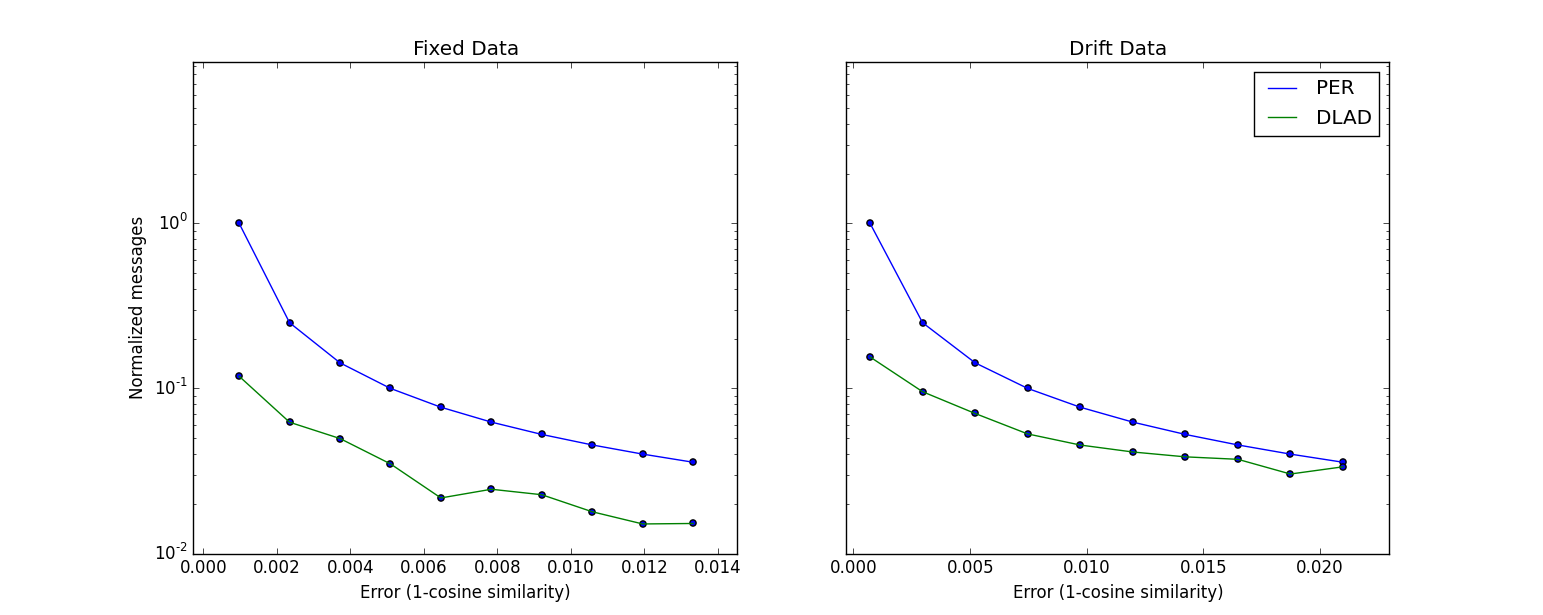
\includegraphics[width=\textwidth]{PER/PERvsDLDAoverError.png}
	\caption{One node naive sync.png}
	\label{PERvsDLDAoverError}
	\end{figure*}

	\begin{figure*}[ht]
	\centering
	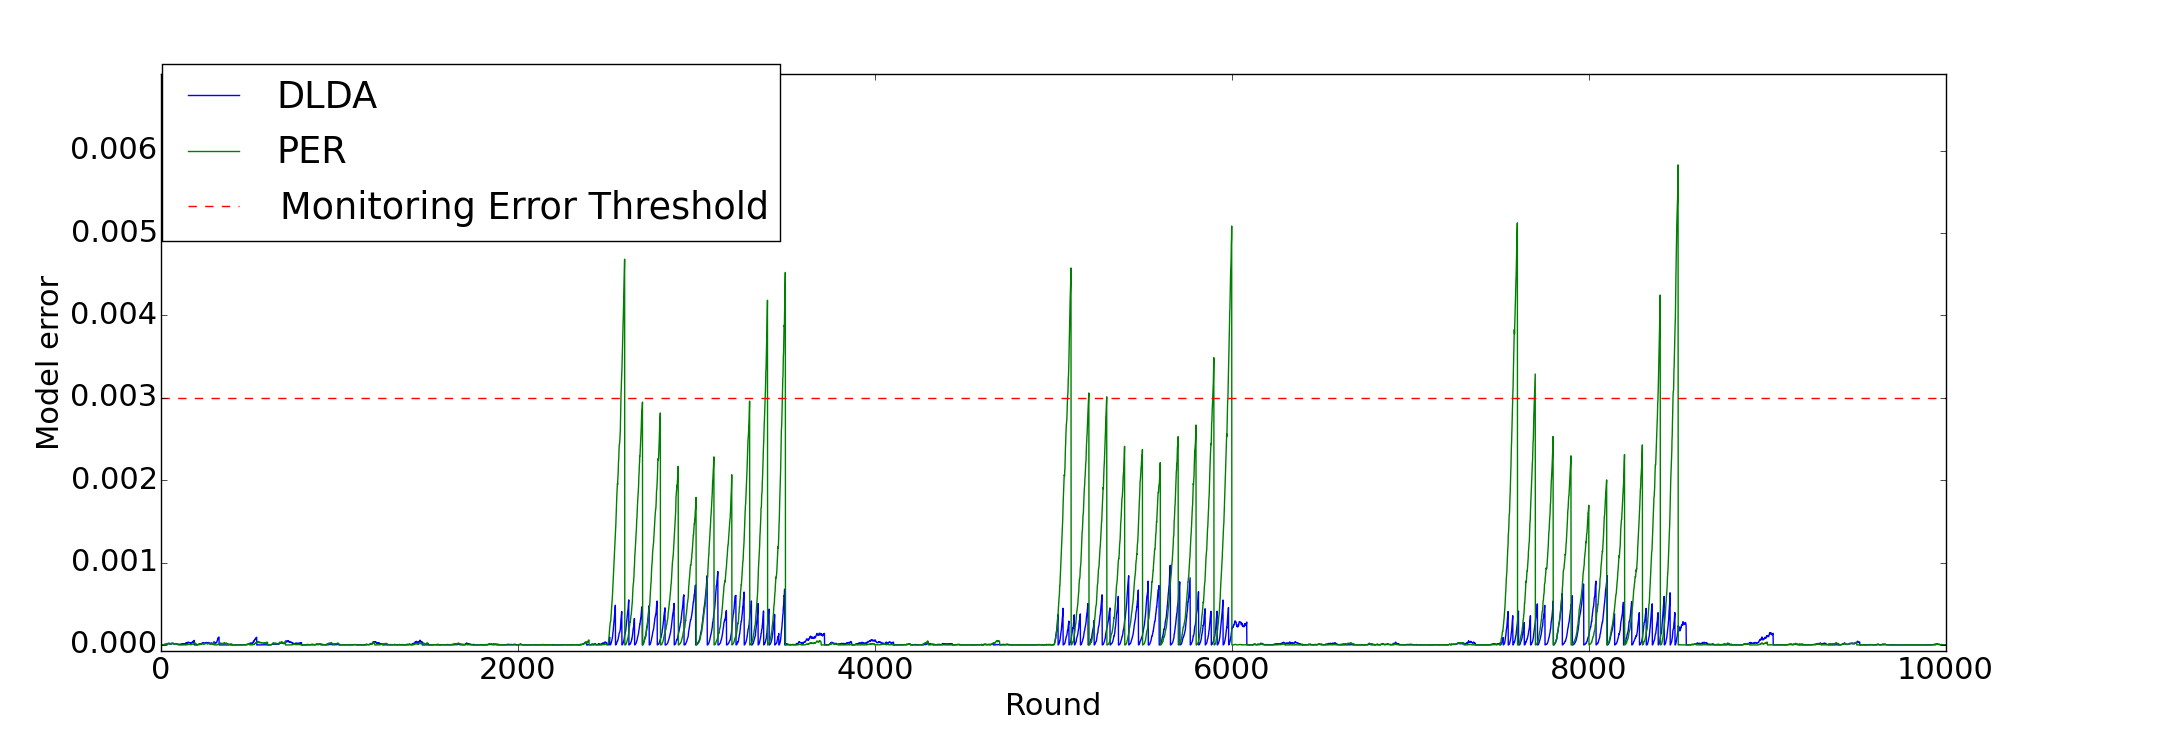
\includegraphics[width=\textwidth]{PER/PERvsDLDAoverTime.png}
	\caption{One node naive sync.png}
	\label{PERvsDLDAoverTime}
	\end{figure*}
\subsubsection{Scalability}
Is seen in Fig \ref{Nodes}.
	\begin{figure}[h]
	\centering
	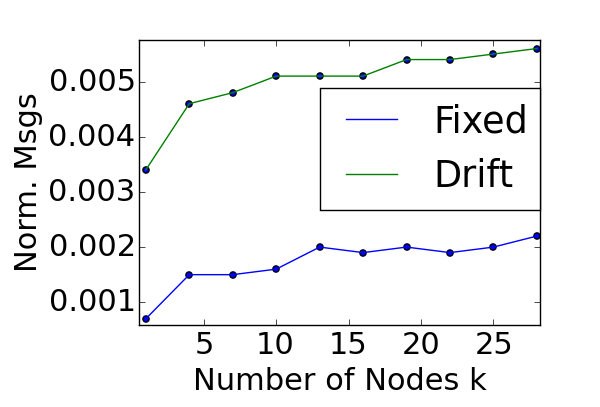
\includegraphics[width=60mm]{CommunicationOfFixedVsDrift/Nodes.png}
	\caption{Communication As Function Of the amount of nodes}
	\label{Nodes}
	\end{figure}
\subsubsection{Dimension}
Is seen in Fig \ref{Dimension}.
	\begin{figure}[h]
	\centering
	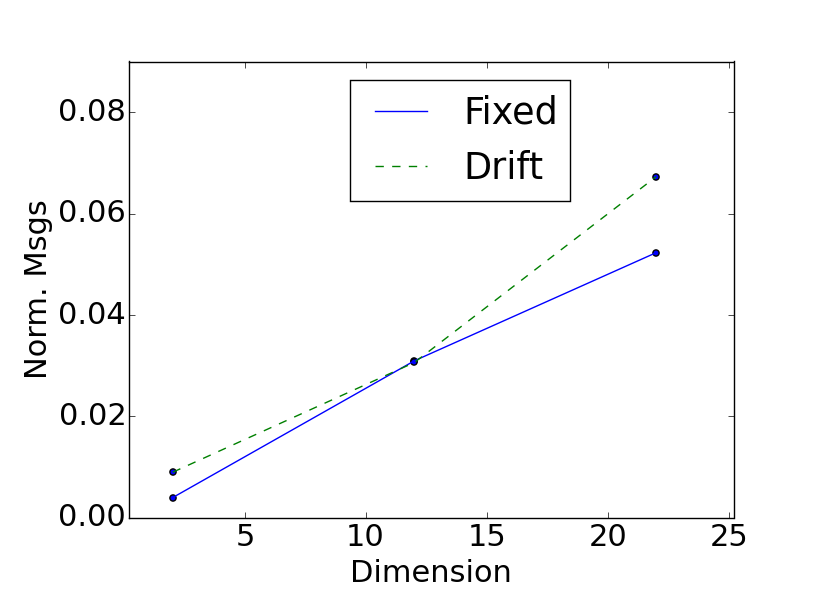
\includegraphics[width=60mm]{CommunicationOfFixedVsDrift/Dimension.png}
	\caption{Communication As Function Of the input's dimension}
	\label{Dimension}
	\end{figure}
\subsubsection{Window Size}
Is seen in Fig \ref{WindowSize}.
	\begin{figure}[h]
	\centering
	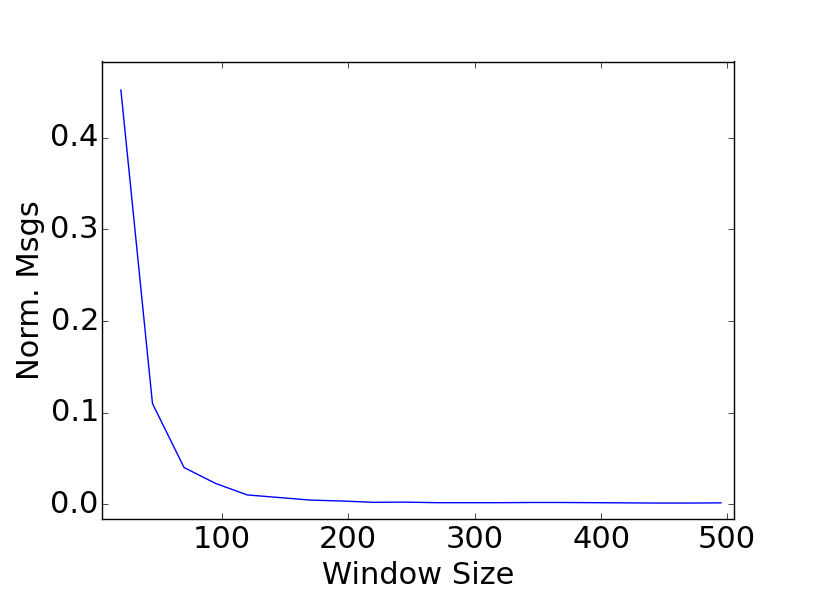
\includegraphics[width=60mm]{CommunicationOfFixedVsDrift/WindowSize.png}
	\caption{Communication As Function Of Window Size}
	\label{WindowSize}
	\end{figure}
\subsubsection{Noise}
Is seen in Fig \ref{Noise}.
	\begin{figure}[h]
	\centering
	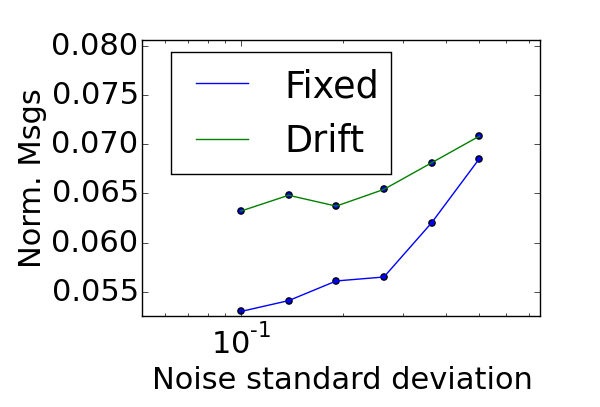
\includegraphics[width=60mm]{CommunicationOfFixedVsDrift/Noise.png}
	\caption{Communication As Function Of standard deviation of the Gaussians that
	generates the data}
	\label{Noise}
	\end{figure}
\end{document}
